\subsection{Esquema de la base de datos}

    A continuación se muestra el esquema de la base de datos donde se observan las relaciones que hay entre las distintas entidades. En su diseño se ha tenido en cuenta que hay dos partes diferenciadas que necesitan un punto de unión:

    \begin{itemize}
        \item Zona del usuario

            Un usuario tendrá sus propios frigríficos y productos asociados a él

        \item Zona comunitaria

            En la zona comunitaria se crearán los supermercados y productos asociados a cada uno. Así, un usuario agregará a su frigoríficos los productos que de forma colaborativa se han guardado en la plataforma.

        \item Punto de unión

            La tabla \emph{my\_compra\_producto} enlaza entre un producto agregado por un usuario a una compra, al supermercado al que pertenece ese producto y que producto del supermercado es.

            Además, en esta tabla, se duplican todos los datos del producto del supermercado. De esta manera, se puede editar el precio del producto del supermercado y para un usuario; para tal compra; ese precio se mantiene.
    \end{itemize}

\begin{figure}[H]
    \centering
    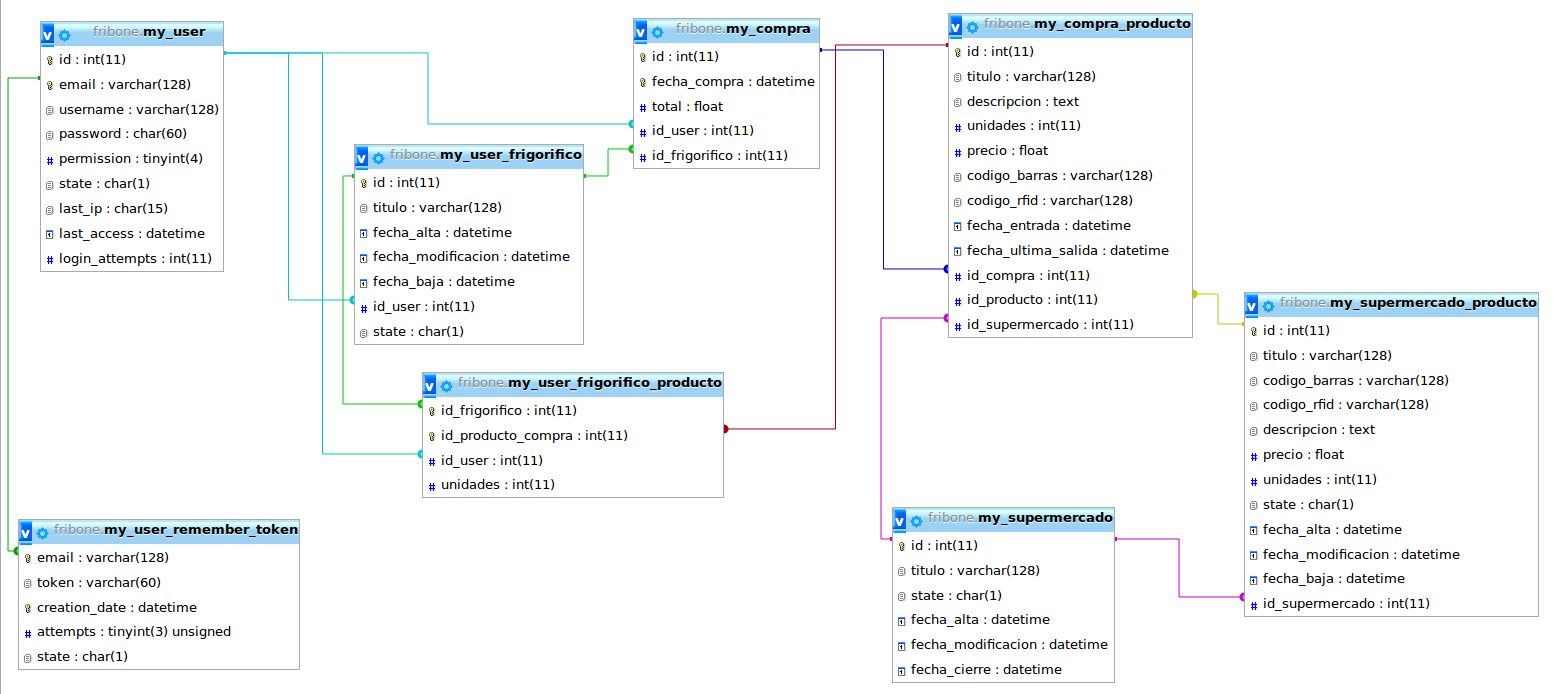
\includegraphics[keepaspectratio,width=0.9\textwidth]{esquema-bd.png}
    \caption{Esquema de la base de datos}\label{fig:esquema-bd}
\end{figure}
